\section{Обхождане на графа}

\subsection{Алгоритми}

\paragraph*{} Резултатът от обхождането на графа е гора от дървета, като всяко дърво е представено като корен и списък от наредени двойки \textit{(родител, дете)}. Списъкът е сортиран в реда в който DFS алгоритъмът е намерил съответното дете. Може да има повече от едно дърво ако графът не е свързан. Имплементирани са три различни DFS алгоритъма.

\paragraph*{Seq} Стандартен еднонишков dfs алгоритъм. Използва се за база за сравнение.

\paragraph*{Cheat} За всеки връх се създава задача, която пуска dfs от този връх, и задачите се добавят в thread pool-а. Това значи че в началото ще започнат $t$ на брой задачи - но една за всяка нишка. Когато задача приключи ще се извика следващата на нейно място (която най-вероятно ще види че върха от който почва вече е обходен и ще приключи).

Използва се споделен масив за проверка на това кои върхове са обходени. Първата нишка, която намери връх го маркира за обходен. Ако нишка види вече обходен връх тя го игнорира.

Резултатът от алгоритъма се различава от този на стандартния еднонишков варант, защото графът се разделя изкуствено на няколко части. За сметка на това се печели скорост, защото синхронизацията е минимална и отделните нишки не се застъпват в работата, която вършат.

\paragraph*{Par} Пуска се еднонишков dfs алгоритъм, който изпълнява само "спускането". Ако в момента сме във връх $u$  то се преминава към първото необходено дете на $u$. Ако $u$ няма необходени деца, алгоритъма спира. Резултатът от това е стек с всички намерени по време на спускането върхове. Следващата стъпка е връщането назад (backtracking) - при което трябва да се проверят и останалите необходени деца (след първото) на елементите в стека. Тази стъпка се изпълнява паралелно. За всеки елемент от стека се създава подзадача, която изпълнява нормален (пълен) dfs започвайки от този връх. Задачите се добавят в thread pool.

Така пуснатите задачи все още могат да намерят едни и същи върхове. Затова всеки пуснат dfs има цифров приоритет, като dfs-ите с елементи от началото на стека имат по-голям приоритет. Пази се споделен масив, в който за всеки намерен връх се записва приоритета, с който е намерен. Когато една нишка намери връх, тя проверява в масива с приоритетите. Ако този елемент вече съществува с по-голям приоритет, той се смята за обходен и се игнорира. Ако не съществува или има по-малък приоритет, то приоритета се презаписва с по-големия и обхождането продължава.

След приключване на втората стъпка имаме отделни дървета от всяка под-задача. Последната стъпка включва премахване на елементи, които са били обходени повече от веднъж от всички дървета освен това с най-голям приоритет и обединяването на всички дървета в едно. Времето за тези операции е незначително спрямо по-горните стъпки.

Ако след приключването на целият алгоритъм от един връх все още има необходени върхове в графа, алгоритъма се повтаря за тях. Това се случва последователно. Тука не се цели паралелизъм, защото за случаен граф е много вероятно целият или почти целият граф да е една свързана компонента.

Този алгоритъм връща същия резултат като еднонишков dfs. Идеята му е подзадачите да се пуснат в реда в който минимално ще припокриват работата си, което в случая значи задачите с по-голям приоритет да работят преди задачите с по-малък.

\subsection{Резултати}

\paragraph*{} Отново алгоритмите са тествани с два различни входа - генериран ориентиран граф с 200\_000 върха, 4\_000\_000 ребра и 200\_000 върха, 40\_000\_000 ребра.

Понеже \verb|Par| алгоритъма има последователна стъпка максималното достижимо ускорение не е линейно. По измервания отношението (\textit{време за "спускане" / време за изпълнение на seq}) $\approx 0.15$. Затова за идеална ускорение е използвана графиката на $1 / (0.15 + {0.85 \over t})$.

\paragraph*{par - списъци на съседство}

\begin{center}
\begin{tabular}{ c | c c c | c c c | }
  нишки & време (200k/4m) & $S_p$ & $E_p$ & време (200k/40m) & $S_p$ & $E_p$ \\
  \hline
  seq & 0.096 сек & - & - & 0.624 сек & - & - \\
  1  & 1.141 сек & 0.08 & 0.08 & 2.398 сек & 0.26 & 0.26 \\
  2  & 0.642 сек & 0.14 & 0.07 & 1.535 сек & 0.40 & 0.20 \\
  3  & 0.452 сек & 0.21 & 0.07 & 1.087 сек & 0.57 & 0.19 \\
  4  & 0.362 сек & 0.26 & 0.06 & 0.942 сек & 0.66 & 0.16 \\
  6  & 0.250 сек & 0.38 & 0.06 & 0.754 сек & 0.82 & 0.13 \\
  8  & 0.224 сек & 0.42 & 0.05 & 0.444 сек & 1.40 & 0.17 \\
  10 & 0.198 сек & 0.48 & 0.04 & 0.320 сек & 1.94 & 0.19 \\
  12 & 0.190 сек & 0.50 & 0.04 & 0.282 сек & 2.21 & 0.18 \\
  14 & 0.183 сек & 0.52 & 0.03 & 0.244 сек & 2.55 & 0.18 \\
  16 & 0.165 сек & 0.57 & 0.03 & 0.268 сек & 2.32 & 0.14 \\
  20 & 0.179 сек & 0.53 & 0.02 & 0.238 сек & 2.61 & 0.13 \\
  24 & 0.179 сек & 0.53 & 0.02 & 0.238 сек & 2.61 & 0.10 \\
  28 & 0.194 сек & 0.49 & 0.01 & 0.245 сек & 2.54 & 0.09 \\
  32 & 0.197 сек & 0.48 & 0.01 & 0.258 сек & 2.41 & 0.07 \\
\end{tabular}
\end{center}

\begin{figure}[H]
  \centering
  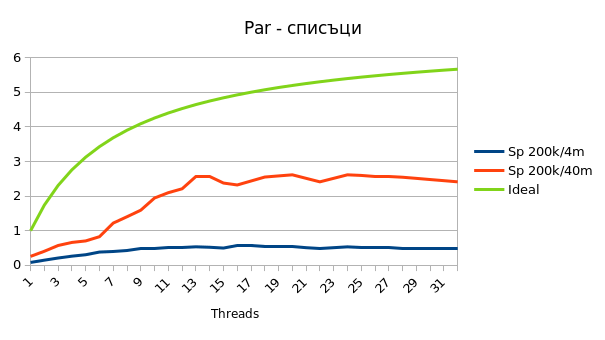
\includegraphics[width=\textwidth]{par_lists.png}
\end{figure}

\paragraph*{par - матрица на съседство}

\begin{center}
\begin{tabular}{ c | c c c | c c c | }
  нишки & време (200k/4m) & $S_p$ & $E_p$ & време (200k/40m) & $S_p$ & $E_p$ \\
  \hline
  seq & 2.175 сек & - & - & 3.072 сек & - & - \\
  1  & 3.621 сек & 0.60 & 0.60 & 6.054 сек & 0.50 &  0.50 \\
  2  & 2.525 сек & 0.86 & 0.43 & 3.954 сек & 0.77 &  0.38 \\
  3  & 2.118 сек & 1.02 & 0.34 & 3.202 сек & 0.95 &  0.31 \\
  4  & 1.805 сек & 1.20 & 0.30 & 2.689 сек & 1.14 &  0.28 \\
  6  & 1.722 сек & 1.26 & 0.21 & 2.296 сек & 1.33 &  0.22 \\
  8  & 1.627 сек & 1.33 & 0.16 & 2.035 сек & 1.50 &  0.18 \\
  10 & 1.599 сек & 1.36 & 0.13 & 2.030 сек & 1.51 &  0.15 \\
  12 & 1.622 сек & 1.34 & 0.11 & 1.881 сек & 1.63 &  0.13 \\
  14 & 1.639 сек & 1.32 & 0.09 & 1.835 сек & 1.67 &  0.11 \\
  16 & 1.666 сек & 1.30 & 0.08 & 1.807 сек & 1.70 &  0.10 \\
  20 & 1.734 сек & 1.25 & 0.06 & 1.782 сек & 1.72 &  0.08 \\
  24 & 1.716 сек & 1.26 & 0.05 & 1.759 сек & 1.74 &  0.07 \\
  28 & 1.979 сек & 1.09 & 0.03 & 1.777 сек & 1.72 &  0.06 \\
  32 & 1.905 сек & 1.14 & 0.03 & 1.805 сек & 1.70 &  0.05 \\
\end{tabular}
\end{center}

\begin{figure}[H]
  \centering
  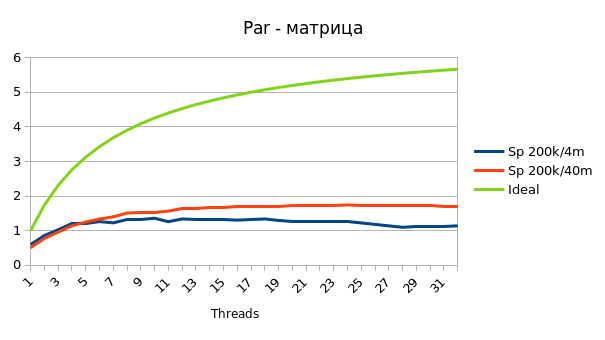
\includegraphics[width=\textwidth]{par_matrix.png}
\end{figure}

\paragraph*{cheat - списъци на съседство}

\begin{center}
\begin{tabular}{ c | c c c | c c c | }
  нишки & време (200k/4m) & $S_p$ & $E_p$ & време (200k/40m) & $S_p$ & $E_p$ \\
  \hline
  seq & 0.099 сек & - & - & 0.584 сек & - & - \\
  1  & 0.165 сек & 0.59 & 0.59 & 1.029 сек & 0.56 & 0.56 \\
  2  & 0.086 сек & 1.14 & 0.57 & 0.650 сек & 0.89 & 0.44 \\
  3  & 0.052 сек & 1.89 & 0.63 & 0.448 сек & 1.30 & 0.43 \\
  4  & 0.044 сек & 2.21 & 0.55 & 0.369 сек & 1.58 & 0.39 \\
  6  & 0.034 сек & 2.90 & 0.48 & 0.264 сек & 2.21 & 0.36 \\
  8  & 0.030 сек & 3.27 & 0.40 & 0.097 сек & 5.99 & 0.74 \\
  10 & 0.029 сек & 3.39 & 0.33 & 0.082 сек & 7.07 & 0.70 \\
  12 & 0.027 сек & 3.57 & 0.29 & 0.072 сек & 8.12 & 0.67 \\
  14 & 0.027 сек & 3.66 & 0.26 & 0.070 сек & 8.28 & 0.59 \\
  16 & 0.026 сек & 3.77 & 0.23 & 0.066 сек & 8.80 & 0.55 \\
  20 & 0.024 сек & 4.02 & 0.20 & 0.070 сек & 8.30 & 0.41 \\
  24 & 0.024 сек & 3.99 & 0.16 & 0.060 сек & 9.65 & 0.40 \\
  28 & 0.027 сек & 3.67 & 0.13 & 0.063 сек & 9.25 & 0.33 \\
  32 & 0.028 сек & 3.42 & 0.10 & 0.065 сек & 8.96 & 0.28 \\
\end{tabular}
\end{center}

\begin{figure}[H]
  \centering
  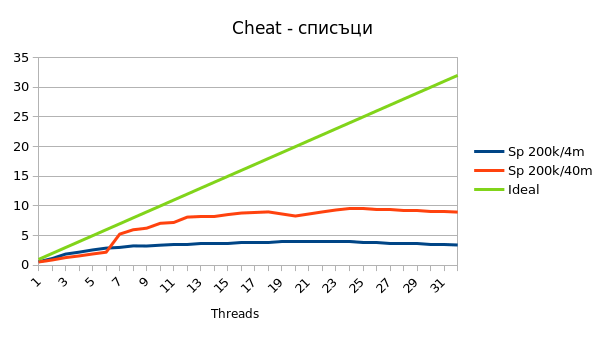
\includegraphics[width=\textwidth]{cheat_lists.png}
\end{figure}

\paragraph*{cheat - матрица на съседство}

\begin{center}
\begin{tabular}{ c | c c c | c c c | }
  нишки & време (200k/4m) & $S_p$ & $E_p$ & време (200k/40m) & $S_p$ & $E_p$ \\
  \hline
  seq & 2.264 сек & - & - & 3.131 сек & - & - \\
  1  & 2.237 сек & 1.01 & 1.011 & 3.515 сек & 0.89 & 0.89 \\
  2  & 1.220 сек & 1.85 & 0.927 & 2.063 сек & 1.51 & 0.75 \\
  3  & 0.950 сек & 2.38 & 0.794 & 1.257 сек & 2.49 & 0.83 \\
  4  & 0.627 сек & 3.60 & 0.901 & 1.009 сек & 3.10 & 0.77 \\
  6  & 0.465 сек & 4.86 & 0.810 & 0.670 сек & 4.66 & 0.77 \\
  8  & 0.330 сек & 6.85 & 0.856 & 0.523 сек & 5.98 & 0.74 \\
  10 & 0.277 сек & 8.15 & 0.815 & 0.427 сек & 7.32 & 0.73 \\
  12 & 0.258 сек & 8.75 & 0.729 & 0.404 сек & 7.73 & 0.64 \\
  14 & 0.223 сек & 10.1 & 0.722 & 0.358 сек & 8.73 & 0.62 \\
  16 & 0.236 сек & 9.55 & 0.597 & 0.328 сек & 9.53 & 0.59 \\
  20 & 0.207 сек & 10.8 & 0.544 & 0.252 сек & 12.4 & 0.62 \\
  24 & 0.207 сек & 10.8 & 0.453 & 0.252 сек & 12.4 & 0.51 \\
  28 & 0.198 сек & 11.4 & 0.407 & 0.251 сек & 12.4 & 0.44 \\
  32 & 0.212 сек & 10.6 & 0.332 & 0.240 сек & 13.0 & 0.40 \\
\end{tabular}
\end{center}

\begin{figure}[H]
  \centering
  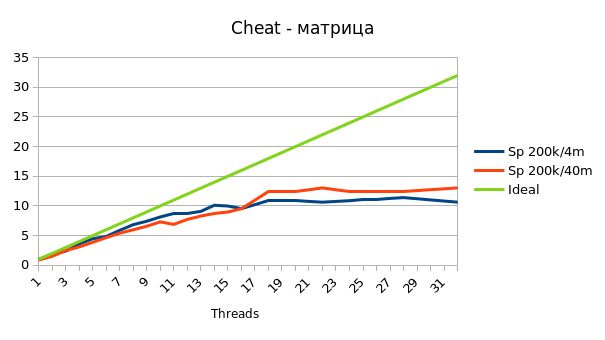
\includegraphics[width=\textwidth]{cheat_matrix.png}
\end{figure}
